\documentclass[12pt]{article}
\usepackage{fullpage,enumitem,amsmath,amssymb,graphicx,listings,color,pdfpages,natbib}
\definecolor{mygreen}{RGB}{28,172,0}  % color values Red, Green, Blue
\definecolor{mylilas}{RGB}{170,55,241}

\begin{document}

\begin{center}
{\Large CS221 Fall 2018 Project} \\
{\Large An AI agent for Lunar Lander}

\begin{tabular}{rl}
Collaborators: & Amey Naik, Prabhjot Singh Rai, Abhishek Bharani \\
SU Net IDs: & ameynaik, prabhjot, abharani
\end{tabular}
\end{center}


\section{Introduction}

The purpose of this project is to build an AI agent to play Lunar Lander game to safely land on a landing pad. We will utilize different variants of DQN such as Double DQN\citep{DoubleQ-learning}, DQN with prioritize replay\citep{PrioritizedReplay} , Dueling network architecture \citep{Dueling}, continuous action space \citep{Continuous} to solve this problem.Our goal is to obtain a policy that once followed by the agent, makes it capable of obtaining scores comparable to human playing  the game  (Oracle).

\section{Problem Statement}
Landing pad is always at coordinates (0,0). Coordinates are the first two numbers in state vector. Reward for moving from the top of the screen to landing pad and zero speed is about 100..140 points. If lander moves away from landing pad it loses reward back. Episode finishes if the lander crashes or comes to rest, receiving additional -100 or +100 points. Each leg ground contact is +10. Firing main engine is -0.3 points each frame. Solved is 200 points. Landing outside landing pad is possible. Fuel is infinite, so an agent can learn to fly and then land on its first attempt. Four discrete actions available: do nothing, fire left orientation engine, fire main engine, fire right orientation engine. The AI agent gets 8 inputs. The eight inputs are mapped to the horizontal position (x-axis), vertical position (y-axis), orientation (theta), linear velocity (v), angular velocity (w), state of each landing leg (left and right), and a “crash” state.
\begin{center}
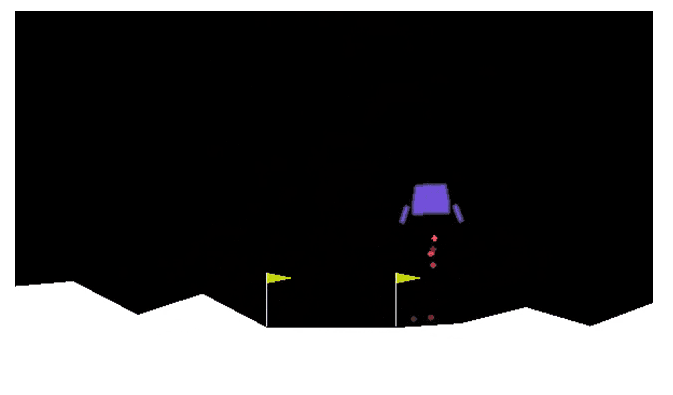
\includegraphics[scale=0.5]{LunarLanderDemoImage.png}
\end{center}

\section{Baseline}
We define multiple baselines for this problem in the increasing order of their performance:
\begin{enumerate}[label=(\alph*)]
\item Taking random actions multiple times till the lunar-lander lands. From the histogram shown below we can see that it never works [add image]
\item Start with randomly picking an action for a new state that is explored, if the state gets explored in the episode ‘e1’, then in the next episode ‘e2’ if you encounter that state, pick the previously stored action for that state. Our baseline will be a greedy algorithm which will act to  fetch maximum rewards but does not account for future states and early convergence.
\end{enumerate}


\section{Oracle}
We define multiple oracles for this problem in the increasing order of their performance and complexity:
\begin{enumerate}[label=(\alph*)]
\item Comparable human playing score.
\item For scoring - an oracle score is the maximum score one can achieve which is 140 [reach landing pad]  + 100 [stopping without crashing] + 10*(num legs) [each leg ground contact].
\item For an agent - if the time-taken to learn and get an average score of 200, the oracle can be the score from the leaderboard available online for this game. [insert link]
\end{enumerate}

\section{Metrics}
We will measure the performance of agent by looking at the average rewards collected in a given number of episodes and the time it takes to obtain optimum \textbf{states}???. There is leader-board to compare the performance of our model against others. \citep{leaderboard}
\newline
 The number of episodes required to earn a minimum of 200+ points (on average), which is an indicator of how fast is the learning.\newline
Also the max score we can achieve? (200-240)


\section{Challenges}
\begin{enumerate}[label=(\alph*)]
\item How fast we learn i.e. with the least number of episodes. Need generalized features such that it doesn’t overfit for a particular episode. Reflex-based DNN will be used here.
\item This problem has a very large state space (\textbf{fill this})MDP (state-based), RL (Q-learning, DQN) , DNN (reflex based)
\end{enumerate}

\bibliography{biblio}
\bibliographystyle{abbrv}

\end{document}